\documentclass[12pts, a4paper]{article}

\usepackage{sujitkc}


\title{Language Definitions}
\author{
  Sujit Kumar Chakrabarti\\
  \texttt{sujitkc@iiitb.ac.in}
}

\date{January 2025}

\begin{document}
\maketitle

\section{API Specification Language}

\subsection{Abstract Syntax}
\begin{figure}
\begin{tabular}{l @{$\rightarrow$\hspace{1cm}} p{10cm}}
\hline
$spec$ & ($g$ : $Decl\star$, $t$: $TypeDecl\star$, $i$ : $Init$, $f$ : $Function\star$, $a$ : $API\star$) \\
$Decl$ & ($v$ : $String$, $t$ : $TypeExpr$) \\
$TypeDecl$ & $VariantDecl$ $|$ $RecordDecl$ \\
$VariantDecl$ & $VariantConstructor+$ \\
$TypeConstructor$ & ($constrname$ : $String$, $TypeExpr\star$) \\
$RecordDecl$ & $recname$ : $String$, $fields$ : $Decl+$ \\
$TypeExpr$ 	&	\vspace{.1cm}
			\begin{minipage}{0.6\textwidth}
		   $TypeConst$ $|$ $TypeVariable$ \\
           $|$ $FuncType$ \\
           $|$ $MapType$ \\
           $|$ $TupleType$ \\
           $|$ $SetType$ \\
           \end{minipage} \\

$TypeConst$ & $String$ \\
$FuncType$ & ($args$: $TypeExpr\star$, $ret$: $TypeExpr$) \\
$MapType$ & ($key$: $TypeExpr$, $val$: $TypeExpr$) \\
$TupleType$ & ($elements$: $TypeExpr+$) \\
$SetType$ & ($elttype$ : $TypeExpr$) \\
$Init$ & ($v$ : $String$, $e$ : $Expr$) \\
\hline
\multicolumn{2}{c}{Functions} \\
\hline
$FunctionDecl$ & ($fname$ : String, $pars$ : $Decl*$, $ret$ : $HTTPResponseCode$, $resp$ : $TypeExpr$) \\
\hline
\multicolumn{2}{c}{APIs} \\
\hline
$API$ & ($pre$ : $Expr$, $call$: $FuncCall$, $resp$ : ($ret$ : $HTTPResponseCode$, $resp$ :  $post$: $Expr$) \\
\hline
\end{tabular}

%Expr::=
%    BinExpr
%  | Var
%  | FuncCall
%
%BinExpr ::= (op: BinOp, Bil : Expr, r : Expr)
%
%BinOp ::= NotIn | In | AND | OR | EQUAL | NOTEQUAL
%
%FuncCall::= FuncName : String,  ArgList : Expr*
%
%Var: (vname : String)
\caption{Abstract Syntax: (a) API Specification Language; (b) Abstract Test Case Language; (c) Common Parts}
\label{f:abssyn}
\end{figure}

\subsection{Example}
\subsection{Example Specification -- Signup-Login API}
\begin{center}
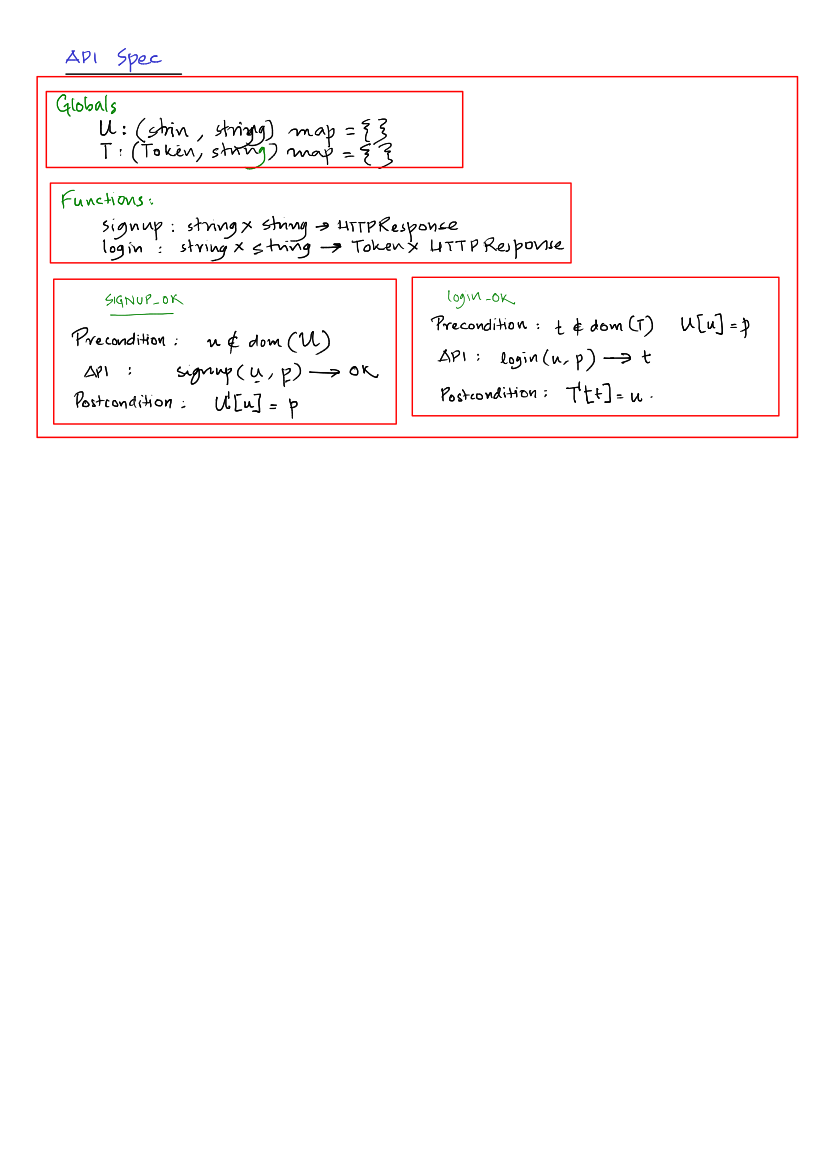
\includegraphics[width=0.6\textwidth]{../images/spec-AST-1.png}
\end{center}
\subsubsection{Abstract Syntax Tree}
\begin{center}
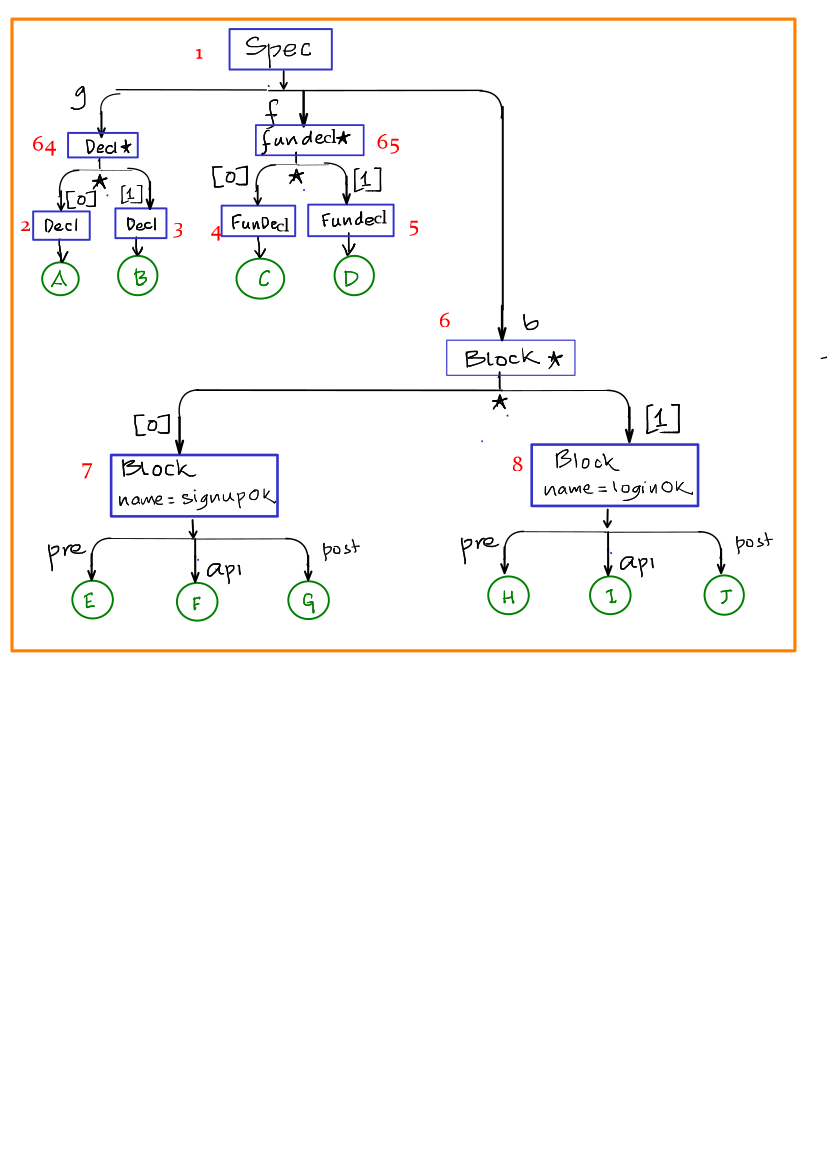
\includegraphics[width=0.9\textwidth]{../images/spec-AST-2.png}
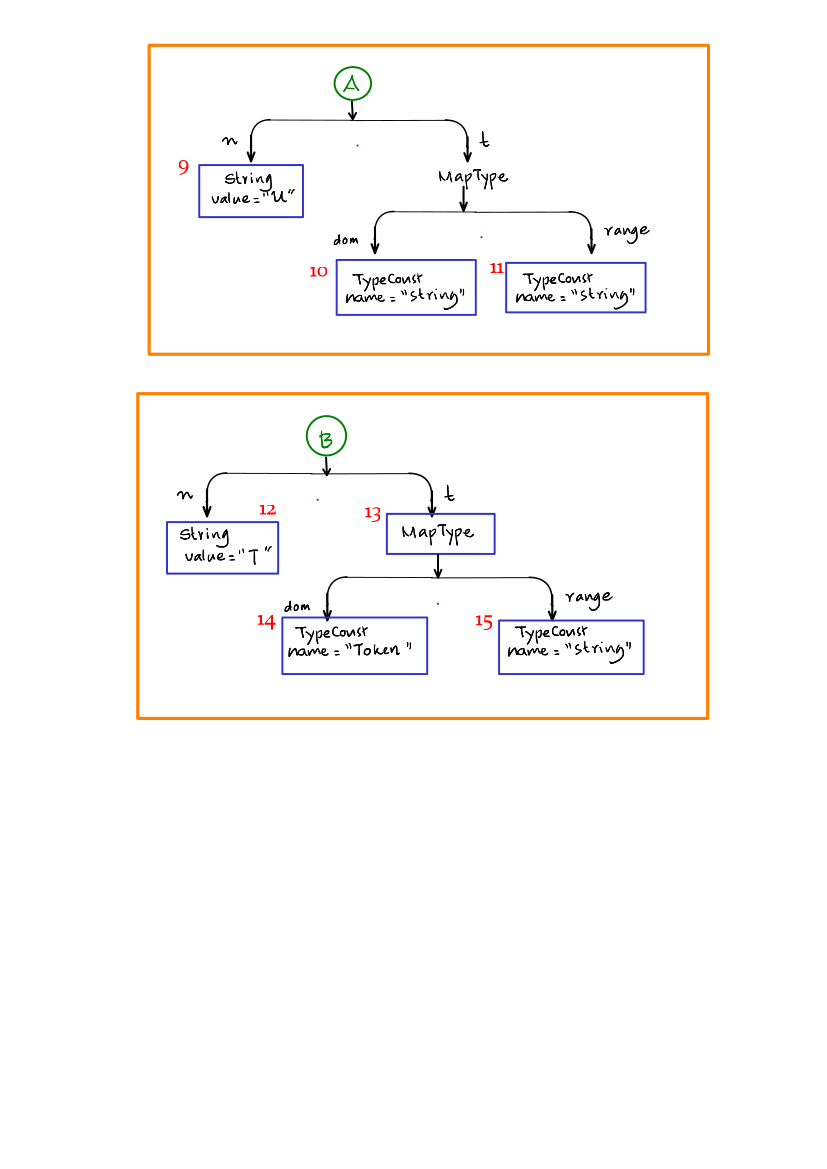
\includegraphics[width=0.9\textwidth]{../images/spec-AST-3.png}
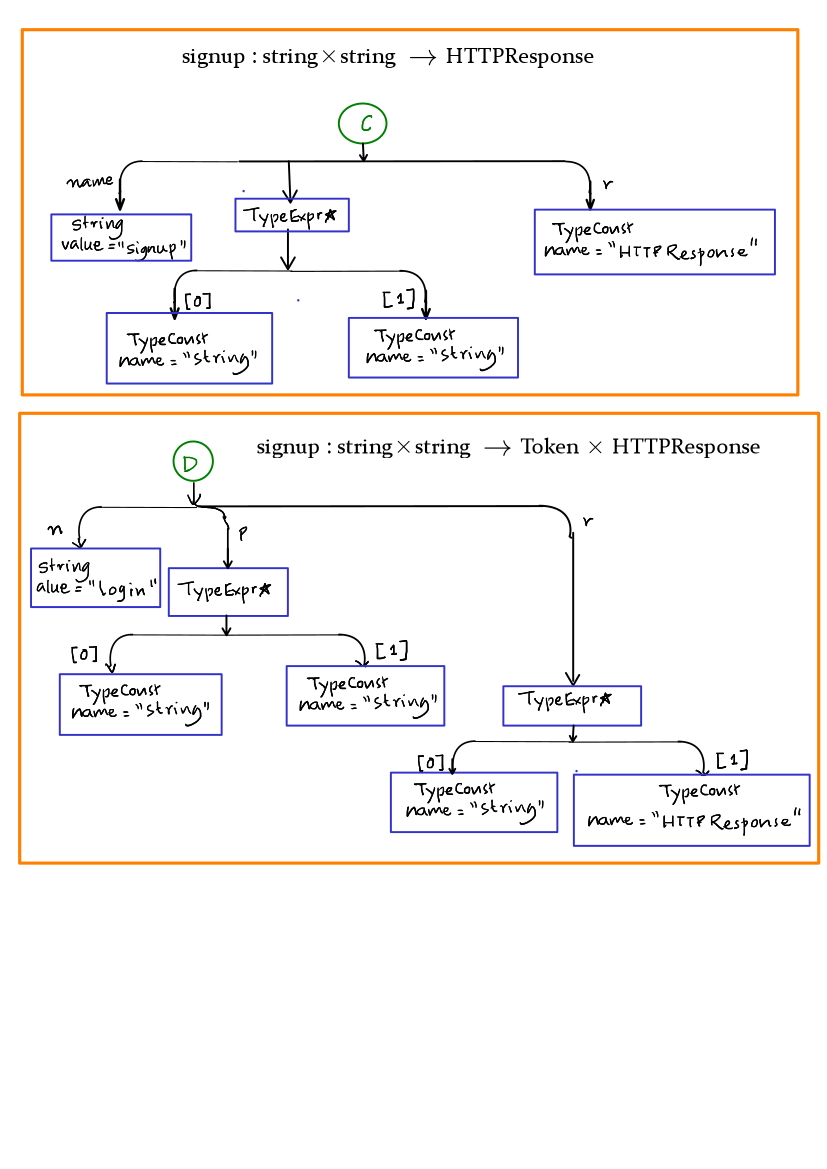
\includegraphics[width=0.9\textwidth]{../images/spec-AST-4.png}
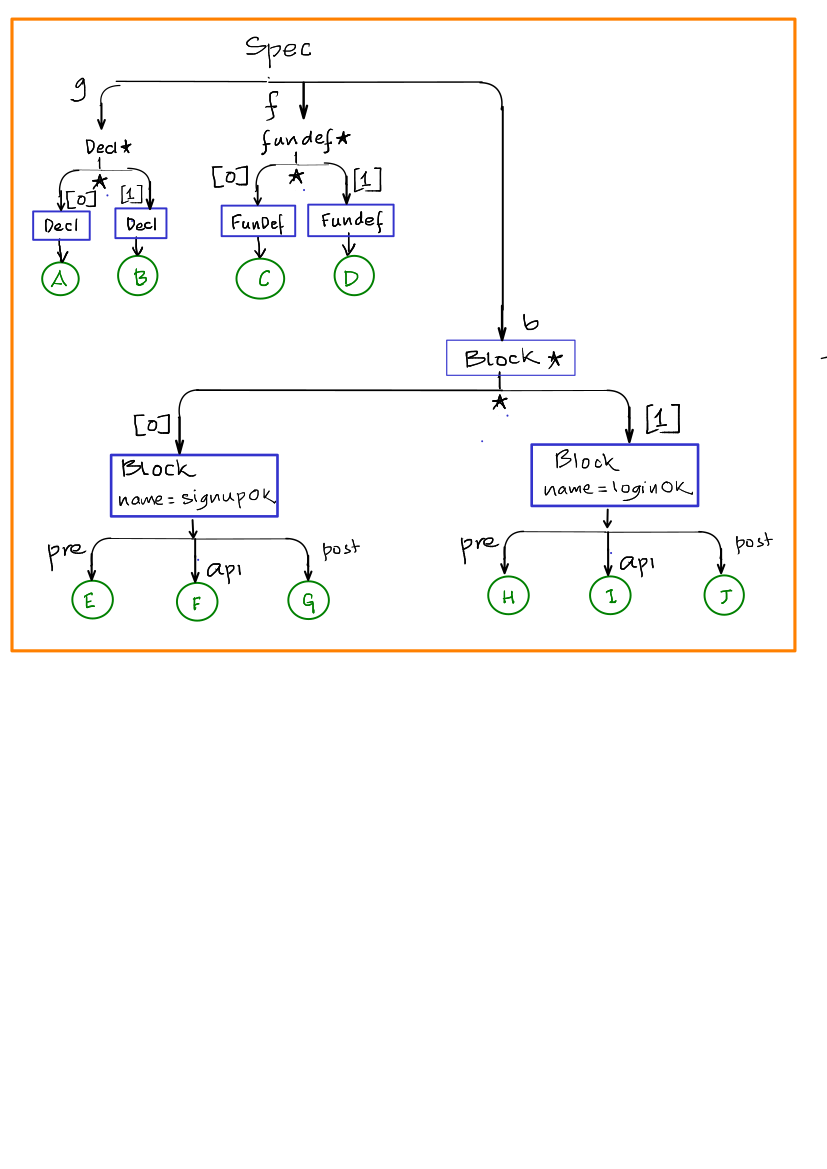
\includegraphics[width=0.9\textwidth]{../images/spec-AST-5.png}
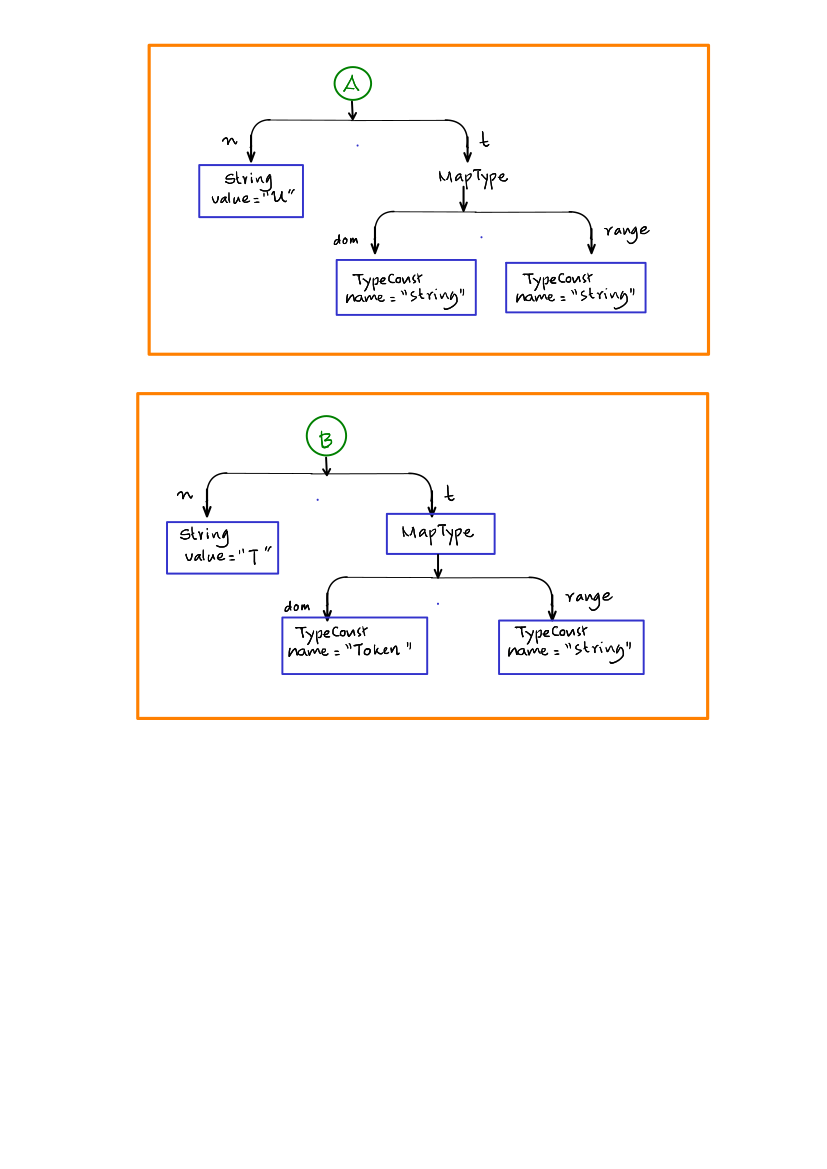
\includegraphics[width=0.9\textwidth]{../images/spec-AST-6.png}
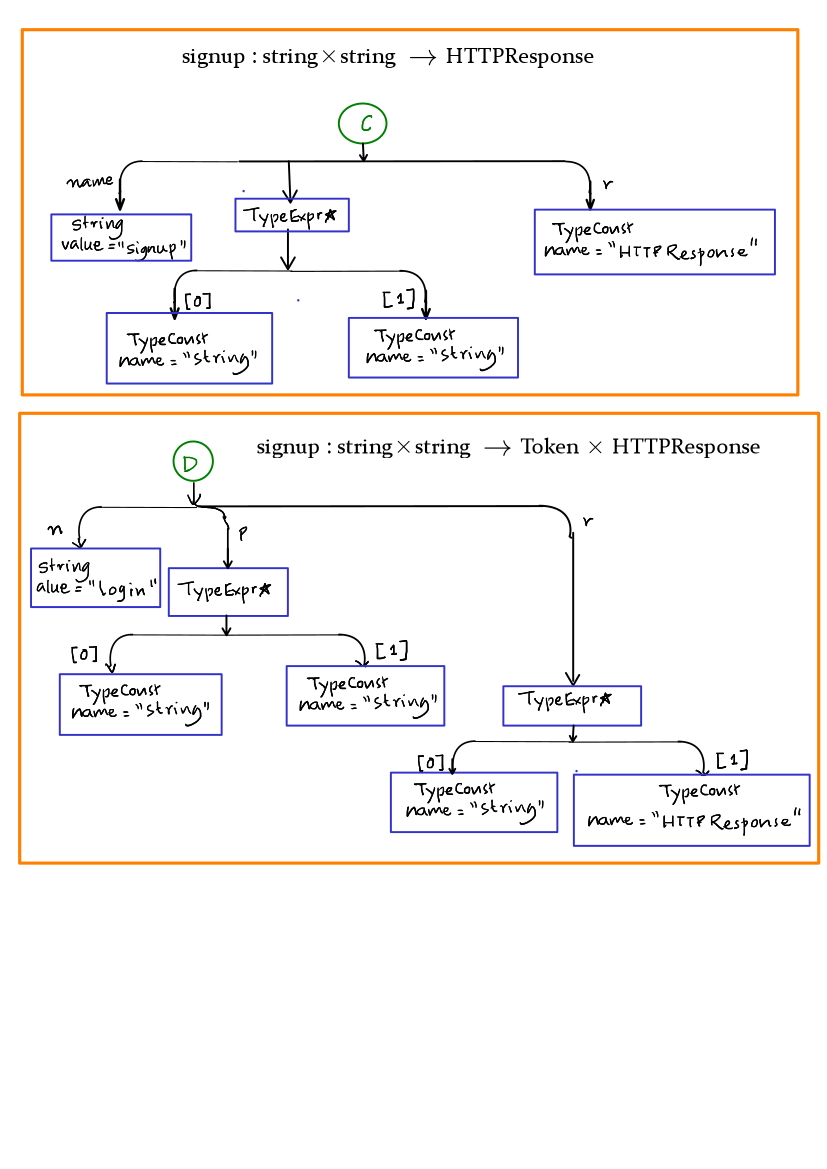
\includegraphics[width=0.9\textwidth]{../images/spec-AST-7.png}
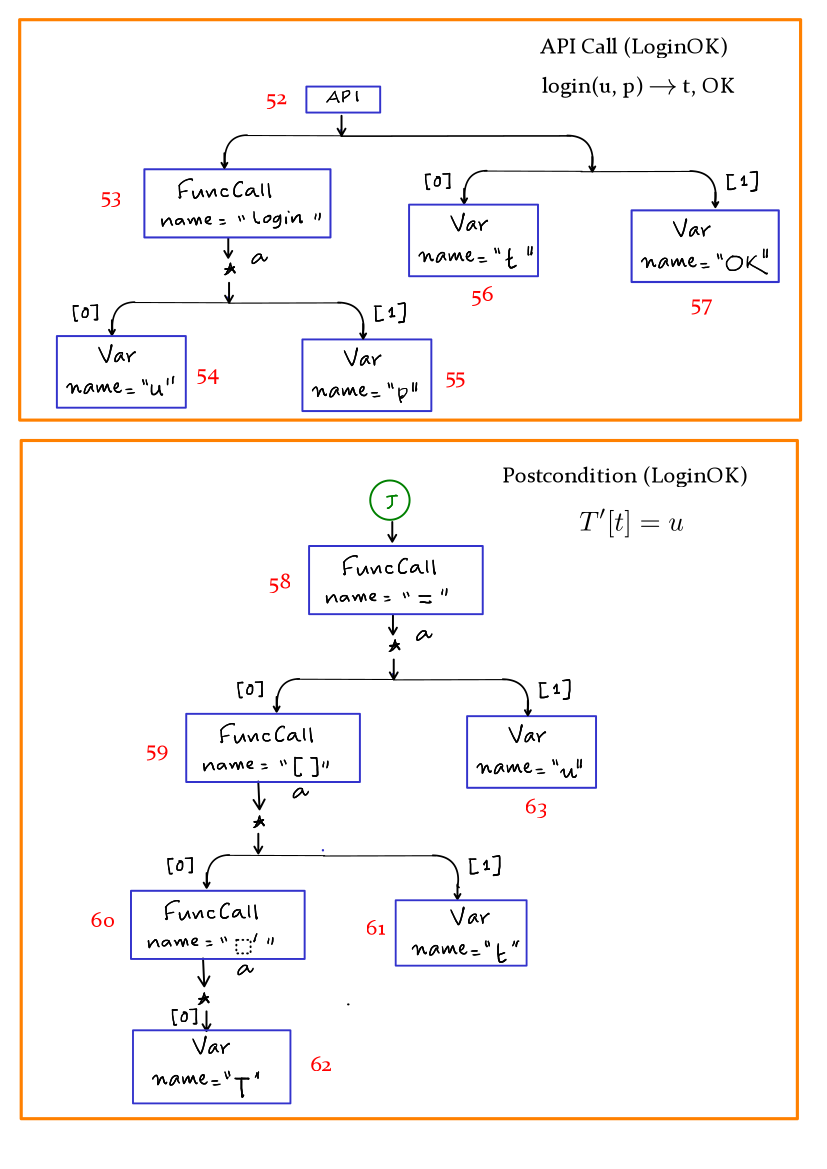
\includegraphics[width=0.9\textwidth]{../images/spec-AST-8.png}
\end{center}
\end{document}
